\chapter{Previous Work and the Problem Set}
\label{ch:previous}

A brewery wastewater train is a computer-controlled plant whose product is a legal discharge, not beer. The beer has already been made. What remains is the water that touched the product and the equipment: wort losses, yeast, spent filter aid, and, in sharp pulses, the acid, caustic, and detergent from clean-in-place. The plant that receives this water must remove organic load and solids and then release the water. Fans sit in the middle of that duty. Blowers supply the oxygen without which the aerobic biomass stops, and exhaust fans keep equalization and flotation from turning anaerobic and odorous. This chapter reviews what is already known about those two technical problems, fan control under a predictive law and oxygen-transfer sensing under a changing wastewater matrix, and then writes the problem this thesis actually solves. The review is selective. It keeps the results that constrain a brewery design and drops municipal detail that does not survive contact with a batch production calendar.

\section{Research on predictive control of aeration fans}
\label{sec:prev-mpc}

\subsection{Where the electricity goes}

Aeration is the largest electrical load in a conventional biological treatment plant. Long-term plant audits put the share of aeration in the range of roughly half to three quarters of the site electricity, with the exact fraction depending on whether sludge handling and pumping are large \cite{longo2016,epa2010energy,amand2013review}. The mechanism is not subtle. Oxygen is only sparingly soluble, the saturation concentration in warm water is near \SI{8}{\milli\gram\per\litre}, and the biomass can consume oxygen faster than diffusion across a quiescent surface can replace it. Machines are therefore used to create interfacial area. In a diffused-air tank the machines are fans in the engineering sense: centrifugal or turbo blowers that raise air from atmospheric pressure to the header pressure set by submergence, diffuser loss, and pipe friction \cite{mueller2002aeration,rosso2008state,tchobanoglous2014}.

Brewery wastewater makes the same machines work harder for three reasons that the municipal literature treats as side cases. The water is warm, often above \SI{30}{\celsius}, so saturation is lower and the driving force $C^{*}-C$ shrinks \cite{simate2011,fillaudeau2006}. The organic load per cubic metre is high, so the oxygen uptake per cubic metre is high even after anaerobic pretreatment \cite{ashraf2021,werkneh2019,batstone2002adm1}. And the clean-in-place chemicals are surfactants. Surfactants are the classical reason the field transfer rate falls below the clean-water test \cite{rosso2006alpha,mueller2002aeration}. A controller that was tuned on a municipal diurnal curve, with a constant transfer factor, is therefore solving a different disturbance problem from the one a brewery automation system actually has.

The standard description of the transfer rate is the two-film expression used in design manuals and in the ASCE clean-water test \cite{asce2007oxygen,pittoors2014,gillot2005}. In the mixed liquor,
\begin{equation}
\label{eq:otr}
\mathrm{OTR}
=
\alpha\,
K_La_{20}
\left(
\beta\,C^{*}_{T}-C
\right)
\theta^{\,T-20},
\end{equation}
where $K_La_{20}$ is the clean-water coefficient at the reference temperature, $\alpha$ is the ratio of process-water to clean-water transfer, $\beta$ corrects saturation for dissolved solids, $\theta\approx 1.024$, and $C$ is the measured dissolved oxygen. The clean-water coefficient itself grows with airflow, but not linearly. For fine-bubble grids a power below one is the usual empirical shape \cite{gillot2005,wagner1998},
\begin{equation}
\label{eq:kla-air}
K_La_{20}
=
k_{0}
\left(\frac{q}{q_{\mathrm{ref}}}\right)^{b},
\qquad
0.7 \le b \le 1,
\end{equation}
with $b$ nearer $0.8$ than $1$ once the floor is already well covered. Equation~\eqref{eq:otr} is the load the fans must meet. Equation~\eqref{eq:kla-air} is the map from that load back to airflow. Everything in later chapters is a way of choosing $q$, and of knowing $\alpha$, so that \eqref{eq:otr} tracks the biological uptake without a large surplus.

A second, easily missed, fan duty sits upstream of the aerobic tank. Equalization of brewery waste is not optional. Flow and pH swing with the clean-in-place program, and a balancing tank of the order of half a day to a day of average flow is the usual first process volume \cite{fillaudeau2006,simate2011}. Warm, strong liquor in that tank goes septic if it is not mixed and lightly aerated, and the room around a dissolved-air flotation unit needs exhaust. Those fans move much less air than the blowers, and their power is a small fraction of blower power, but they are part of the same automation system: they must start and stop with level, hydrogen sulfide, and occupancy, and they must not be forgotten when the blower optimizer is written. This thesis keeps them in the architecture and in the energy account, and it does not pretend they are the main optimization variable.

\subsection{The fan as a constrained machine}

A centrifugal blower is not a valve. It has a map. At a fixed speed the pressure rise falls as flow rises, and below a surge flow the compression system becomes unstable \cite{gravdahl1999surge,dixon2014turbo}. Variable-frequency drives move the map. The fan laws, which follow from kinematic similarity when the machine is not choked and the gas is the same, are
\begin{align}
\frac{q}{q_{0}}
&=
\frac{\omega}{\omega_{0}},
&
\frac{\Delta p}{\Delta p_{0}}
&=
\left(\frac{\omega}{\omega_{0}}\right)^{2},
&
\frac{P_{\mathrm{shaft}}}{P_{\mathrm{shaft},0}}
&=
\left(\frac{\omega}{\omega_{0}}\right)^{3}.
\label{eq:fanlaws}
\end{align}
They are the right local model when speed is the only change. They are the wrong global model for an aeration header, because the discharge pressure is set mostly by the hydrostatic head of the tank, not by the fan curve. Submergence of five metres is about \SI{49}{\kilo\pascal} before diffuser and pipe losses. That head hardly changes with flow. Pipe friction does. A useful header model is therefore
\begin{equation}
\label{eq:header-dp}
\Delta p(q)
=
\Delta p_{\mathrm{static}}
+
c_{f}\,q^{2},
\end{equation}
and the electrical power follows from polytropic compression of the delivered mass flow,
\begin{equation}
\label{eq:polytropic}
P
=
\frac{1}{\eta}
\,
\dot{m}\,
\frac{\gamma}{\gamma-1}\,
R_{\mathrm{sp}} T_{\mathrm{in}}
\left[
\left(\frac{p_{\mathrm{out}}}{p_{\mathrm{in}}}\right)^{(\gamma-1)/\gamma}
-
1
\right],
\end{equation}
with $p_{\mathrm{out}}=p_{\mathrm{in}}+\Delta p(q)$ and $\eta$ the product of polytropic, motor, and drive efficiencies \cite{dixon2014turbo,iec60034}. Equation~\eqref{eq:polytropic} is much closer to linear in $q$ than the pure cube law, because $\Delta p$ is nearly constant. A controller that saves energy by the cube law alone will overstate the value of small speed reductions and understate the value of not running an extra machine.

Staging is the hybrid part of the problem. Three blowers on one header, which is a common small-plant arrangement, give a discrete decision $n\in\{1,2,3\}$ and a continuous speed for the machines that are on. Running three machines at low speed can cross the surge line of each machine even when the header flow is moderate. Running one machine at high speed can meet the same header flow at a better surge margin and a better efficiency, until that machine hits its motor limit and a second machine must start. The start itself has a cost: inrush, a pressure bump in the header, and wear. Hybrid model predictive control was built for exactly this mixture of logic and continuous dynamics \cite{bemporad1999hybrid}. Cristea and co-workers used a hybrid nonlinear predictive law on an aeration problem and showed that the on--off structure of the air supply can be carried inside the optimizer rather than left to a separate sequencer \cite{cristea2011}. What that work does not carry is a brewery calendar, and what it does not protect explicitly is the surge margin of a centrifugal map. Both omissions matter once the fans are real machines rather than a smooth airflow input.

\subsection{From on--off dissolved-oxygen control to predictive laws}

The control literature on aeration is large and, in its later part, repetitive. The review by {\AA}mand, Olsson, and Carlsson is the clean map of the older half: manual valves, time clocks, on--off bands around a dissolved-oxygen sensor, then proportional-integral control of airflow or of blower pressure, then cascade structures in which an outer dissolved-oxygen loop writes an airflow set-point to an inner flow loop \cite{amand2013review,olsson2012ica,olsson2005ica}. Cascade is the structure still shipped with most blower panels. It is the right inner loop. It is a poor outer loop when the load jumps faster than the oxygen sensor and the blower can settle, and when the set-point itself is a number an operator picked once and then left alone.

A standard discrete proportional-integral law for the outer loop is
\begin{equation}
\label{eq:pi}
q_{k}
=
q_{\mathrm{bias}}
+
K_{P}\,e_{k}
+
K_{I}\sum_{i=0}^{k} e_{i}\,\Delta t,
\qquad
e_{k}
=
C_{\mathrm{sp}}-C_{k},
\end{equation}
with anti-windup on the sum \cite{astrom2006pid,skogestad2003pid,seborg2016}. The bias $q_{\mathrm{bias}}$ is where the fan sits when the error is zero. If the bias is wrong, the integral removes the offset, slowly. During a clean-in-place slug the integral is still carrying the bias from the previous hour. The fan is late on the way up and late on the way down. That pattern, not the gain formula, is the operational defect.

Ammonia-based aeration control moves the outer set-point. Instead of holding a fixed dissolved-oxygen number, a slower loop raises or lowers $C_{\mathrm{sp}}$ so that effluent ammonia stays near a low target, which avoids aerating for nitrification the plant does not need \cite{rieger2014abac,amand2012optimal,samuelsson2007}. The idea is right for municipal nitrogen permits. A brewery polishing tank is often carbon-limited, and the permit that bites is chemical oxygen demand, biochemical oxygen demand, and solids. Ammonia feedback is still useful as a floor: if dissolved oxygen is allowed to fall so far that nitrification stops, ammonia walks out of the tank even when the carbon looks acceptable. Rieger and co-workers also make a point this thesis uses. Feedforward from influent ammonia helps when the load swing is unusual. When the swing is ordinary, feedback is enough \cite{rieger2014abac}. A brewery clean-in-place dump is the unusual swing, and it is unusual on a clock the factory already owns.

Model predictive control enters the aeration literature as a way to use a dynamic model instead of a fixed set-point. Holenda and co-workers applied a predictive law to dissolved oxygen on an activated-sludge model and showed tighter control than a linear regulator on the same plant model \cite{holenda2008}. Shen, Chen, and Corriou put predictive control on the BSM1 benchmark and compared it with the default proportional-integral strategy of that benchmark \cite{shen2008,copp2002cost,jeppsson2004cost}. Ostace, Cristea, and Agachi used a modified ASM1 inside a predictive controller aimed at operating cost \cite{ostace2011,henze1987asm1,henze2000asm}. Vega and co-workers separated set-point optimization from the tracking predictive layer, which is the classical two-layer pattern of process control \cite{vega2014,engell2007,darby2011rto}. Zeng and Liu formulated an economic predictive controller directly on BSM1, so that effluent quality and operating cost enter the stage cost instead of entering only through a set-point chosen elsewhere \cite{zeng2015empc,ellis2014empc}. Revollar and co-workers compared economic predictive strategies on the same family of plants \cite{revollar2017}. Sant{\'i}n, Pedret, and Vilanova showed that a variable dissolved-oxygen set-point, computed at a higher layer, removes effluent violations that a fixed set-point leaves behind, and they compared fuzzy and predictive configurations for that job \cite{santin2015jpc,santin2015iecr}.

The plant models under these controllers are the IWA activated-sludge models and the benchmark plants built from them \cite{henze1987asm1,henze2000asm,gernaey2004state,gernaey2014benchmarking,nopens2010bsm2}. For the oxygen balance in one aerated tank the ASM1 skeleton is
\begin{equation}
\label{eq:asm1-do}
\frac{\mathrm{d}C}{\mathrm{d}t}
=
\frac{Q}{V}\bigl(C_{\mathrm{in}}-C\bigr)
+
K_La\,(C^{*}_{\infty}-C)
-
\mathrm{OUR}(S,C,X),
\end{equation}
with $\mathrm{OUR}$ the sum of heterotrophic growth, decay, and nitrification. The benchmark cost indices then integrate effluent ammonia, total nitrogen, suspended solids, chemical oxygen demand, and biochemical oxygen demand into an effluent quality index, and they integrate aeration energy and pumping energy into an operating cost \cite{vanrolleghem2002,copp2002cost,nopens2010bsm2}. Those indices are the right language for a comparison. They are the wrong disturbance. BSM1 influent is a municipal file with a daily and weekly shape. It does not contain a surfactant pulse tied to a clean-in-place recipe, and its aeration input is an oxygen-transfer coefficient, not a fan with a surge line \cite{schraa2017}.

Hierarchical predictive control, as in the work of Brdys and of Piotrowski, already splits the problem in the way a real plant must be split: a slow optimizer writes set-points, and fast loops move valves and machines \cite{brdys2008,piotrowski2008}. O'Brien and co-workers report a plant trial of predictive aeration control and record the practical issues, among them model error and the need to keep the existing safety interlocks \cite{obrien2011}. Iratni and Chang survey the later control literature and list the same open issues: sensors, model mismatch, and the gap between a benchmark file and a plant that an operator will leave in automatic \cite{iratni2019}. Stare and co-workers compared nitrogen-removal strategies on operating cost and showed that the ranking of controllers depends on the price of electricity and on the effluent weights, which is a warning against quoting a single percentage as if it were a property of the algorithm \cite{stare2007}.

The predictive-control textbook results that this thesis relies on are standard and should be named as such. Offset-free tracking needs a disturbance model or an integrator, otherwise a constant model error becomes a constant dissolved-oxygen error \cite{pannocchia2003offset,rawlings2017mpc,maciejowski2002}. Recursive feasibility and stability of a constrained predictive law need a terminal cost or a terminal set, or a shorter argument that the problem solved online is a descent on a control Lyapunov function \cite{mayne2000mpc,qin2003mpc,garcia1989mpc,camacho2007mpc}. Real-time solution of the resulting nonlinear program is a software problem that is now routine at the time scales of aeration, which are minutes, not milliseconds \cite{diehl2002nmpc,andersson2019casadi,wachter2006ipopt,nocedal2006,boyd2004convex}. None of that machinery, by itself, knows that a brewery will dump a fermenter in forty minutes.

\begin{figure}[ht]
\centering
\begin{tikzpicture}[
  font=\small,
  box/.style={draw, rounded corners=2pt, align=center, minimum height=8mm, inner sep=3pt},
  arr/.style={-{Stealth[length=2mm]}, thick}
]
\node[box, fill=blue!8] (sp) {Operator\\DO set-point};
\node[box, fill=blue!8, right=8mm of sp] (pi) {PI\\outer loop};
\node[box, fill=orange!12, right=8mm of pi] (fc) {Airflow\\PI};
\node[box, fill=orange!12, right=8mm of fc] (vfd) {Blower\\drive};
\node[box, fill=green!10, below=9mm of fc] (tank) {Aerobic tank};
\node[box, fill=red!8, below=9mm of pi] (do) {DO probe};
\draw[arr] (sp) -- (pi);
\draw[arr] (pi) -- node[above,font=\scriptsize]{$q_{\mathrm{sp}}$} (fc);
\draw[arr] (fc) -- (vfd);
\draw[arr] (vfd) -- node[right,font=\scriptsize,pos=0.3]{air} (vfd |- tank) -- (tank);
\draw[arr] (tank) -- (do);
\draw[arr] (do) -- (pi);
\end{tikzpicture}
\caption{Cascade dissolved-oxygen control as it is usually installed. The outer loop does not see the production calendar, and the blower drive does not see a surge constraint from the optimizer. Both limits are outside this diagram on purpose: they are the gap Chapter~\ref{ch:method} closes.}
\label{fig:cascade-classical}
\end{figure}

\subsection{What the fan-control literature does not give a brewery}

The gap can be stated without a new slogan. Published predictive aeration controllers, including the hybrid and economic ones cited above, optimize a transfer coefficient or an airflow for a municipal load. They do not ingest a batch production schedule as a known disturbance trajectory \cite{harjunkoski2014,goode2013fouling,pettigrew2015cip}. They rarely place the centrifugal surge margin inside the same optimization as the dissolved-oxygen limit \cite{gravdahl1999surge,schraa2017}. And they treat $\alpha$ in \eqref{eq:otr} as a calibrated constant, or they hide it inside a black-box gain, which fails when the next disturbance is a detergent. The first technology of this thesis is the controller that fills that gap: a hybrid economic predictive law whose preview comes from the brewery calendar and whose fan model is \eqref{eq:header-dp}--\eqref{eq:polytropic} with an explicit surge inequality. The second technology, reviewed next, is how $\alpha$ is obtained in time to be useful to that law.

\section{Research on physics-informed sensing of oxygen transfer}
\label{sec:prev-sensor}

\subsection{Why a dissolved-oxygen probe is not an oxygen-transfer measurement}

A dissolved-oxygen probe reports $C$ in \eqref{eq:asm1-do}. It does not report $K_La$, $\alpha$, or $\mathrm{OUR}$. Those three quantities appear only as a product and a difference. Rearrangement of a steady balance, ignoring the small advective term, gives
\begin{equation}
\label{eq:unident}
K_La\,(C^{*}_{\infty}-C)
-
\mathrm{OUR}
\approx 0.
\end{equation}
Any pair $(K_La,\mathrm{OUR})$ on that line agrees with the same $C$. A single probe, at a single airflow, cannot separate a surfactant event, which lowers $K_La$, from a load event, which raises $\mathrm{OUR}$. Both make $C$ fall, and a proportional-integral fan loop responds to both by adding air. If the cause was surfactant, extra air is partly right. If the probe itself has fouled and reads low, extra air is waste. Rieger, Alex, and co-workers documented, early, that sensor properties and not only control laws decide whether automatic aeration is trustworthy \cite{rieger2003sensors,olsson2012ica}.

The direct experimental answer is off-gas testing. The oxygen mole fraction in the gas leaving the tank, compared with the air in, gives the oxygen actually transferred, and hence a field $K_La$ and a field efficiency, without assuming the biological rate \cite{redmon1983,leu2009,asce2007oxygen}. Leu, Rosso, Larson, and Stenstrom showed that real-time efficiency monitoring of this kind can be used to cut aeration energy, because the operator stops paying for transfer that the diffuser grid is no longer delivering \cite{leu2009,rosso2008state}. Off-gas hoods are the reference measurement. They are also equipment: hoods, gas sensors, and a maintenance task. A brewery polishing tank can justify them as a calibration tool. It is a weak assumption that every tank, every week, will have a clean hood signal at the moment a clean-in-place slug arrives. A soft sensor that runs on the fan instruments the plant already owns is the practical companion, checked against off-gas when the hood is in service.

\subsection{The surfactant factor}

The $\alpha$ factor is the ratio of process-water to clean-water mass transfer under otherwise matched conditions. Design values near $0.6$ are common for municipal fine-bubble tanks. Rosso and Stenstrom showed that surfactants depress $\alpha$ sharply, and that the depression is worse for fine bubbles than for coarse bubbles because the surfactant occupies the interface that fine bubbles were built to maximize \cite{rosso2006alpha}. Viscosity and high mixed-liquor solids depress transfer again, which is why high-solids tanks need their own correction \cite{krampe2003,mueller2002aeration}. Brewery clean-in-place liquors are a surfactant source by design. The detergents that remove beer stone and biofilm are the same class of molecules that sit on an air bubble \cite{goode2013fouling,pettigrew2015cip,simate2011}. In addition, brewery waste is warm and can carry diatomaceous earth fines from filtration, which abrade and clog diffuser pores and therefore move $k_{0}$ in \eqref{eq:kla-air} as well as $\alpha$ \cite{fillaudeau2006}.

A constant $\alpha$, identified during a quiet week, is then not a conservative design choice. It is an optimistic one. The fan controller that uses it will under-predict the airflow required during the detergent hour and will over-predict it afterward, if the identification is ever updated from that hour alone. The literature already knows the chemistry. It does not, in the control papers cited in Section~\ref{sec:prev-mpc}, close the loop from a live $\alpha$ estimate back into a fan optimizer on a brewery schedule.

\subsection{Soft sensors and what they have been asked to estimate}

Data-derived soft sensors for treatment plants are reviewed by Haimi, Mulas, Corona, and Vahala \cite{haimi2013soft}. The typical target is an effluent concentration that is measured in the laboratory a few times a day: chemical oxygen demand, total nitrogen, or suspended solids. The typical inputs are the online sensors the plant already has. D{\"u}rrenmatt and Gujer compared data-driven model classes for the same operational purpose and stressed that a model which fits a historical record can still be useless to an operator if its inputs are not the decisions the operator can move \cite{durrenmatt2012}. Newhart, Holloway, Hering, and Cath review performance analysis of plants from operating data, and Corominas and co-workers review the step from data to an operational decision \cite{newhart2019,corominas2018}. The shared warning is worth keeping. A soft sensor that is accurate on yesterday's file and silent about its own physics will be believed for a month and then bypassed.

For dissolved oxygen specifically, the prediction problem is easier than effluent chemical oxygen demand, because the probe exists and is simply late, noisy, or drifting. Koksal and Aydin report a hybrid of transfer learning and physics-informed modelling for dissolved-oxygen prediction on an industrial plant, using a simulator as one source of knowledge and another plant as a second source \cite{koksal2024,pan2010transfer}. That paper is the closest published neighbour of the second technology here. It improves a dissolved-oxygen forecast. It does not extract $\alpha$ as a variable to be handed to a fan optimizer, and it does not use a production schedule as an input. Those two uses are the difference this thesis claims.

Classical identification would write a small parameter vector $\theta=(\alpha,k_{0})$ and a state that includes $C$ and a slowly varying oxygen uptake, and would run a recursive estimator \cite{ljung1999,kalman1960,rao2003mhe}. Moving-horizon estimation is the constrained version of that idea and matches the constraints already present in predictive control \cite{rao2003mhe,rawlings2017mpc}. It is the right tool when the parameter dimension is small and the model is trusted. It is brittle when the airflow-to-$K_La$ exponent, the probe bias, and a sudden surfactant step are all wrong together. A physics-informed network is used here not because neural networks are newer, but because the residual of \eqref{eq:asm1-do} can be imposed on a function approximator that also accepts the schedule features a low-order parameter vector does not have room for.

\subsection{Physics-informed models}

A physics-informed neural network trains a differentiable function $u_{\phi}(x)$ so that a differential residual, not only a data error, is small \cite{raissi2019pinn,karniadakis2021piml}. For a scalar residual $r(x,u_{\phi},\partial u_{\phi})$, the training objective has the shape
\begin{equation}
\label{eq:pinn-generic}
\mathcal{L}(\phi)
=
\mathcal{L}_{\mathrm{data}}(\phi)
+
\lambda\,
\mathcal{L}_{\mathrm{phys}}(\phi)
+
\lambda_{b}\,
\mathcal{L}_{\mathrm{bound}}(\phi).
\end{equation}
Raissi, Perdikaris, and Karniadakis demonstrated the pattern on forward and inverse partial differential equations \cite{raissi2019pinn}. Karniadakis and co-workers review the wider programme of physics-informed machine learning \cite{karniadakis2021piml}. The training difficulties are now well described. Gradient conflict between the data term and the residual term produces models that fit the probe and ignore the balance, or the reverse \cite{wang2021gradient,cuomo2022}. Libraries such as DeepXDE make the residual form easy to express \cite{lu2021deepxde}. None of that work is a wastewater paper. The transferrable part is the residual. Here the residual is not a partial differential equation on a spatial mesh. It is the ordinary balance \eqref{eq:asm1-do}, evaluated on the samples the historian already stores, plus algebraic residuals from the fan map \eqref{eq:polytropic} so that a claimed airflow has to agree with the measured power.

Neural differential equations are a second, related form: the network defines a vector field and an integrator produces the trajectory \cite{chen2018node,hochreiter1997lstm,goodfellow2016deep}. They are attractive when the state must be rolled forward over a long horizon. They are heavier than this problem needs at inference time. The fan controller runs on an edge computer on a cycle of one to five minutes. A small residual network that emits $\alpha$, $K_La$, and $\mathrm{OUR}$ in one shot, trained with \eqref{eq:pinn-generic}, meets that cycle. The long short-term memory network remains relevant as a baseline for the data term, which is why it is cited, and it is not the model this thesis asks the operator to trust \cite{hochreiter1997lstm}.

Identifiability still has to be argued, because a network can hide the non-uniqueness of \eqref{eq:unident} inside its weights. The argument used in Chapter~\ref{ch:method} is structural. Airflow and power fix a delivered $q$ through \eqref{eq:polytropic}. The clean-water curve \eqref{eq:kla-air} then fixes $K_La$ up to $\alpha$. The oxygen balance fixes $\mathrm{OUR}$ once $K_La$ and $C$ are known. The schedule feature, which is zero in quiet hours and one during a detergent recipe, gives $\alpha$ a reason to move that is not collinear with a smooth diurnal uptake. When that feature is constant for a long time, the information matrix thins, and the estimator must hold $\alpha$ rather than chase noise. That is a standard excitation requirement \cite{ljung1999}, applied to a plant whose excitation is partly chosen by the production department.

\subsection{What the sensing literature does not give the fan controller}

Off-gas is accurate and scarce. Black-box soft sensors are available and unconstrained by \eqref{eq:otr}. Physics-informed dissolved-oxygen models now exist for industrial wastewater \cite{koksal2024}, and they stop at the forecast of $C$. The missing instrument is a soft sensor whose outputs are the parameters of the fan problem: a live $\alpha$, a live $K_La$, and a live uptake, with a residual that tells the controller when the dissolved-oxygen probe should not be believed. That is the second technology. It is useful only if the first technology has a place to put the numbers. The two reviews are therefore one design.

\begin{figure}[ht]
\centering
\begin{tikzpicture}[
  font=\small,
  box/.style={draw, rounded corners=2pt, align=center, minimum width=28mm, minimum height=9mm, inner sep=2pt},
  gap/.style={draw, dashed, rounded corners=2pt, align=center, minimum width=28mm, minimum height=9mm, inner sep=2pt, fill=yellow!15}
]
\node[box, fill=blue!8] (lit1) at (0,0) {Municipal\\MPC and EMPC};
\node[box, fill=blue!8] (lit2) at (4.6,0) {Hybrid blower\\sequencing};
\node[box, fill=green!10] (lit3) at (0,-2.1) {Off-gas and\\$\alpha$ chemistry};
\node[box, fill=green!10] (lit4) at (4.6,-2.1) {PINN and\\DO soft sensors};
\node[gap] (g1) at (9.4,-1.05) {Brewery gap:\\calendar preview,\\surge-aware fans,\\live $\alpha$ in the law};
\draw[-{Stealth}, thick] (lit1) -- (g1);
\draw[-{Stealth}, thick] (lit2) -- (g1);
\draw[-{Stealth}, thick] (lit3) -- (g1);
\draw[-{Stealth}, thick] (lit4) -- (g1);
\end{tikzpicture}
\caption{The four bodies of work this chapter uses, and the brewery-specific gap they leave. Chapter~\ref{ch:method} puts a schedule-aware fan controller on one side of the gap and a physics-informed transfer sensor on the other.}
\label{fig:gap}
\end{figure}

\section{Problem set}
\label{sec:problem}

\subsection{The plant the controller is responsible for}

The plant considered here is the wastewater cleaning end of a brewery, not the brewhouse. Water that has been used in production is collected, treated, and discharged. Reuse inside the brewery is outside the problem. The train, in process order, is coarse screening, a mixed and lightly aerated equalization tank, pH correction, anaerobic high-rate pretreatment, dissolved-air flotation as a solids buffer, an aerobic polishing tank with fine-bubble diffusion, and a secondary clarifier. Anaerobic pretreatment is included because brewery waste is strong enough that sending it raw to an aerobic tank makes the fan problem artificially impossible; the anaerobic stage is the standard response in the brewery treatment literature \cite{simate2011,ashraf2021,werkneh2019,shao2008asbr,chen2016anmbr,ince2000,batstone2002adm1,bernard2001,nopens2009interface}. The fans this thesis controls are the aerobic blowers and the exhaust fans on equalization and flotation. Pumps, dosing valves, and the clarifier mechanism are in the automation, and they are not the optimization variables of the two technologies.

Table~\ref{tab:train} fixes the representative sizes used from here on. They describe a polishing train after anaerobic pretreatment, sized so that a competent dissolved-oxygen loop can meet the study discharge limit, and so that a constant-speed blower sized for the worst hour wastes a large amount of air in the quiet hours. They are not the nameplate of a particular site.

\begin{table}[ht]
\centering
\caption{Representative cleaning train used as the problem data. Aerobic influent values are after anaerobic pretreatment and refer to the five production regimes of Table~\ref{tab:regimes}.}
\label{tab:train}
\begin{tabular}{@{}ll@{}}
\toprule
Quantity & Value used in this thesis \\
\midrule
Equalization & mixed, detention of several hours, exhaust fan pair \\
Aerobic volume $V$ & \SI{900}{\cubic\metre} \\
Mixed liquor $X$ & \SI{3800}{\milli\gram\per\litre} volatile solids \\
Diffusers & fine bubble, submergence giving about \SI{52}{\kilo\pascal} static head \\
Blowers & three centrifugal machines, variable speed, common header \\
Header capacity & \SI{9000}{\nmcph} \\
Mixing floor & \SI{900}{\nmcph} \\
Inert $\mathrm{COD}$ fraction $f$ & $0.08$ \\
Study discharge limit & \SI{125}{\milli\gram\per\litre} $\mathrm{COD}$ in the clarifier effluent \\
Dissolved-oxygen floor & \SI{1.5}{\milli\gram\per\litre} during production, as an operational constraint \\
\bottomrule
\end{tabular}
\end{table}

The study discharge limit of \SI{125}{\milli\gram\per\litre} chemical oxygen demand is taken as the numerical permit target inside the optimization and the estimation. It is the same order as the secondary-treatment figure used for urban wastewater in the European directive, and it is used here as a study target for a direct discharge, not as a claim that every brewery permit is that number \cite{eu1991uwwtd,tchobanoglous2014}. A site permit can be tighter or can be a sewer ordinance. The controller does not depend on the number $125$. It depends on having a number.

The five regimes in Table~\ref{tab:regimes} are the weekly disturbance. They are a compressed production calendar: a long base load, a brewhouse peak, a fermentation clean-in-place window in which $\alpha$ falls because detergent reaches the aerobic tank, a shorter packaging clean-in-place window, and a weekend hold. Durations sum to $168$ hours. Mean influent flow over the week is $55.5\,\mathrm{m^{3}/h}$ and the flow-weighted mean aerobic influent chemical oxygen demand is about \SI{402}{\milli\gram\per\litre}. Both follow from the table by direct averaging, and both are recomputed in Chapter~\ref{ch:estimate} when energy is normalized.

\begin{table}[ht]
\centering
\caption{Weekly production regimes imposed on the aerobic polishing tank. The factor $\alpha$ is the true plant value. Controllers that assume a constant $\alpha$ do not receive this column.}
\label{tab:regimes}
\begin{tabular}{@{}lrrrrrr@{}}
\toprule
Regime & Hours & $Q$ (\si{\cubic\metre\per\hour}) & $\mathrm{COD}$ (\si{\milli\gram\per\litre}) & TKN & $\alpha$ & $T$ (\si{\celsius}) \\
\midrule
Base production & 96 & 50 & 380 & 26 & 0.60 & 28 \\
Brewhouse peak & 30 & 70 & 460 & 34 & 0.52 & 31 \\
Fermentation CIP & 18 & 75 & 430 & 28 & 0.40 & 33 \\
Packaging CIP & 12 & 68 & 410 & 26 & 0.46 & 30 \\
Weekend hold & 12 & 22 & 160 & 12 & 0.66 & 26 \\
\bottomrule
\end{tabular}
\end{table}

\begin{figure}[ht]
\centering
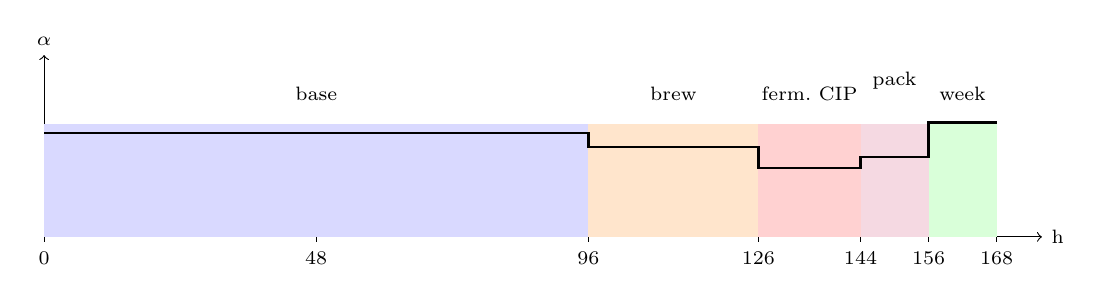
\begin{tikzpicture}[font=\scriptsize, x=0.072cm, y=0.55cm]
  \draw[->] (0,0) -- (176,0) node[right] {h};
  \draw[->] (0,0) -- (0,4.2) node[above] {$\alpha$};
  \foreach \x/\name in {0/0, 48/48, 96/96, 126/126, 144/144, 156/156, 168/168}{
    \draw (\x,0) -- (\x,-0.12) node[below, rotate=0] {\x};
  }
  \fill[blue!15] (0,0) rectangle (96,2.6);
  \fill[orange!20] (96,0) rectangle (126,2.6);
  \fill[red!18] (126,0) rectangle (144,2.6);
  \fill[purple!15] (144,0) rectangle (156,2.6);
  \fill[green!15] (156,0) rectangle (168,2.6);
  \draw[thick] (0,2.40) -- (96,2.40) -- (96,2.08) -- (126,2.08) -- (126,1.60) -- (144,1.60) -- (144,1.84) -- (156,1.84) -- (156,2.64) -- (168,2.64);
  \node at (48,3.3) {base};
  \node at (111,3.3) {brew};
  \node at (135,3.3) {ferm.\ CIP};
  \node at (150,3.6) {pack};
  \node at (162,3.3) {week};
\end{tikzpicture}
\caption{The true oxygen-transfer factor over the representative week. The drop at $126\,\mathrm{h}$ is the fermentation clean-in-place detergent reaching the aerobic tank. A controller that keeps $\alpha=0.55$ is wrong on this interval by about thirty percent.}
\label{fig:alpha-week}
\end{figure}

\subsection{Biological and oxygen balances that define feasibility}

The estimation model, stated here because the problem is not well posed without it, is a single aerobic tank with biodegradable chemical oxygen demand $S_{b}$, inert chemical oxygen demand $S_{i}$, ammonia $S_{n}$, and dissolved oxygen $C$. Mixed-liquor solids $X$ are held by sludge-age control and are an input, not a state. With Monod factors
\begin{equation}
\label{eq:monod}
\mu_{S}
=
\frac{S_{b}}{K_{S}+S_{b}},
\quad
\mu_{C}
=
\frac{C}{K_{\mathrm{DO}}+C},
\quad
\mu_{N}
=
\frac{S_{n}}{K_{N}+S_{n}},
\end{equation}
the rates used throughout this thesis are
\begin{align}
r_{\mathrm{COD}}
&=
q_{\mathrm{COD}}\,X\,\mu_{S}\,\mu_{C},
&
r_{N}
&=
q_{N}\,X\,\mu_{N}\,\mu_{C},
\label{eq:rates}
\end{align}
and the oxygen uptake that the fans must match is
\begin{equation}
\label{eq:our}
\mathrm{OUR}
=
Y_{\mathrm{O_{2},COD}}\,r_{\mathrm{COD}}
+
Y_{\mathrm{O_{2},N}}\,r_{N}.
\end{equation}
The numerical values are $K_{S}=\SI{40}{\milli\gram\per\litre}$, $K_{\mathrm{DO}}=\SI{0.35}{\milli\gram\per\litre}$, $K_{N}=\SI{1}{\milli\gram\per\litre}$, $q_{\mathrm{COD}}=0.0145\,\mathrm{L\,mg^{-1}\,h^{-1}}$, $q_{N}=0.00040\,\mathrm{L\,mg^{-1}\,h^{-1}}$, $Y_{\mathrm{O_{2},COD}}=0.95$, and $Y_{\mathrm{O_{2},N}}=4.57$. The product $q_{\mathrm{COD}}X$ is about \SI{55}{\milli\gram\per\litre\per\hour}, which is the kinetic ceiling. The fan ceiling is lower during the detergent window, and that is intentional: the interesting constraint is oxygen transfer, not a kinetic parameter.

Mass balances close the problem statement:
\begin{align}
\frac{\mathrm{d}S_{b}}{\mathrm{d}t}
&=
\frac{Q}{V}\bigl((1-f)\,\mathrm{COD}_{\mathrm{in}}-S_{b}\bigr)
-
r_{\mathrm{COD}},
\label{eq:sb}\\
\frac{\mathrm{d}S_{i}}{\mathrm{d}t}
&=
\frac{Q}{V}\bigl(f\,\mathrm{COD}_{\mathrm{in}}-S_{i}\bigr),
\label{eq:si}\\
\frac{\mathrm{d}S_{n}}{\mathrm{d}t}
&=
\frac{Q}{V}\bigl(\mathrm{TKN}_{\mathrm{in}}-S_{n}\bigr)
-
r_{N},
\label{eq:sn}\\
\frac{\mathrm{d}C}{\mathrm{d}t}
&=
K_La(\alpha,q,T)\,
\bigl(\beta C^{*}(T)-C\bigr)
-
\mathrm{OUR}.
\label{eq:do-bal}
\end{align}
Effluent chemical oxygen demand is $S_{b}+S_{i}$ after the clarifier has removed solids. The clarifier itself is not dynamically modelled. The Tak{\'a}cs clarifier would be the next model if the permit were on suspended solids rather than on dissolved and colloidal organic load \cite{takacs1991}. For this problem the clarifier is a solids separator that the automation must keep in service, and the organic permit is decided in the aerobic tank.

The transfer coefficient in \eqref{eq:do-bal} is the estimation curve
\begin{equation}
\label{eq:kla-est}
K_La
=
\alpha\,
k_{\mathrm{ref}}
\left(\frac{q}{q_{\mathrm{ref}}}\right)^{0.82}
\theta^{\,T-20},
\end{equation}
with $k_{\mathrm{ref}}=6.5\,\mathrm{h^{-1}}$ at $q_{\mathrm{ref}}=\SI{2500}{\nmcph}$ and $\theta=1.024$. Saturation $C^{*}(T)$ is interpolated from the fresh-water table $8.11$, $7.83$, $7.54$, $7.43$, $7.16\,\mathrm{mg/L}$ at $26$, $28$, $30$, $31$, and \SI{33}{\celsius}. The factor $\beta$ is $0.95$. These numbers are part of the problem data. Changing them changes the absolute kilowatt-hours and should not change the ranking of a schedule-aware law against a law that ignores the schedule, which is the comparison Chapter~\ref{ch:estimate} is built to make.

Fan power is \eqref{eq:polytropic} with the header
\begin{equation}
\label{eq:dp-num}
\Delta p
=
52
+
0.55\left(\frac{q}{1000}\right)^{2}
\quad[\mathrm{kPa}],
\end{equation}
inlet temperature \SI{20}{\celsius}, and $\eta=0.70\times 0.95\times 0.97$. Delivered airflow lags the command with a time constant of $0.10\,\mathrm{h}$, and the probe lags the tank with a time constant of $0.08\,\mathrm{h}$. Those lags are why a purely reactive loop is late, and why a preview of forty-five minutes is long enough to matter.

One steady-state check belongs in the problem statement so that later plots are not the first time the numbers appear. At base load, $Q=\SI{50}{\cubic\metre\per\hour}$, $\mathrm{COD}_{\mathrm{in}}=\SI{380}{\milli\gram\per\litre}$, $f=0.08$, the biodegradable influent is \SI{350}{\milli\gram\per\litre}. With $C=\SI{1.8}{\milli\gram\per\litre}$ the Monod product is high enough that the balance \eqref{eq:sb} settles near $S_{b}\approx\SI{25}{\milli\gram\per\litre}$. Inert chemical oxygen demand settles at $f\,\mathrm{COD}_{\mathrm{in}}=\SI{30}{\milli\gram\per\litre}$. Effluent chemical oxygen demand near \SI{55}{\milli\gram\per\litre} is then the quiet-week target, not a result to be celebrated. The fermentation clean-in-place window, with the same kinetic ceiling and $\alpha=0.40$, settles near \SI{90}{\milli\gram\per\litre} if dissolved oxygen stays near \SI{2}{\milli\gram\per\litre}, and it climbs through the \SI{125}{\milli\gram\per\litre} study limit if dissolved oxygen is held near \SI{0.5}{\milli\gram\per\litre} for a large part of the eighteen hours. The controller's job is to buy the first of those two outcomes with as little fan energy as the surge and mixing constraints allow.

\subsection{The two decision problems}

The technologies are now stated as optimization problems. Time is discrete with step $\Delta t$. The horizon is $N$ steps. The schedule encoder, defined properly in Chapter~\ref{ch:method}, produces a disturbance preview $D_{k:k+N}$ that contains future flow, chemical oxygen demand, temperature, and a detergent flag.

\textbf{Problem P1, fan control.} Given the current state estimate and the preview $D$, choose the binary staging $z_{0:N-1}$ and the continuous commands $u_{0:N-1}$ (fan speeds and the total airflow) to minimize
\begin{equation}
\label{eq:p1}
\sum_{j=0}^{N-1}
\left(
P(q_{j},z_{j})\,\Delta t
+
\lambda_{C}\,\phi_{C}(C_{j})
+
\lambda_{S}\,\phi_{S}(S_{b,j}+S_{i,j})
+
\lambda_{z}\,\abs{z_{j}-z_{j-1}}
\right)
\end{equation}
subject to the discrete form of \eqref{eq:sb}--\eqref{eq:do-bal}, the fan map, the surge inequalities, the box limits on speed and airflow, and the probe-health interlock. The hinge penalties $\phi_{C}$ and $\phi_{S}$ are zero when dissolved oxygen is above its floor and chemical oxygen demand is below the study limit, and they grow linearly beyond those lines. This is an economic predictive problem in the sense of \cite{zeng2015empc,ellis2014empc,rawlings2017mpc}, with a hybrid decision in the sense of \cite{bemporad1999hybrid,cristea2011}.

\textbf{Problem P2, transfer sensing.} Given a window of fan power, airflow, temperature, header pressure, dissolved oxygen, and the same schedule features, choose the network parameters $\phi$ and the latent trajectories of $\alpha$, $K_La$, and $\mathrm{OUR}$ to minimize \eqref{eq:pinn-generic}, where the physics term is the residual of \eqref{eq:do-bal} and a power residual from \eqref{eq:polytropic}. The deployed sensor freezes $\phi$ and runs a short update of the latent state only. P2 is useful insofar as its $\alpha$ and $K_La$ reduce the model error inside P1. A sensor that predicts dissolved oxygen accurately and emits an $\alpha$ the optimizer cannot use has not solved P2 as defined here.

\subsection{Questions the rest of the thesis has to answer}

The design questions are the following.

\begin{enumerate}[leftmargin=1.6em,itemsep=0.4em]
\item Can the production calendar be encoded as a disturbance trajectory that a fan optimizer accepts without a human redrawing set-points at the start of each clean-in-place?
\item Can the blower staging, the surge margin, and the header power model sit inside that optimizer rather than in a separate sequencer that fights it?
\item Can $\alpha$ during a detergent window be estimated from instruments the fan already has, with the oxygen balance enforced, well enough that the optimizer stops using the quiet-week value?
\item On the representative week of Table~\ref{tab:regimes}, how much blower energy does the combined law use relative to constant speed, to a competent dissolved-oxygen proportional-integral loop at a fixed set-point of \SI{2.5}{\milli\gram\per\litre}, and to a predictive inversion that keeps $\alpha$ at $0.55$ and does not read the calendar?
\item Which of those savings survive the mixing floor, the blower lag, and a soft-sensor lag of a few tenths of an hour?
\end{enumerate}

The questions are system questions. They are answered by a specification in Chapter~\ref{ch:method} and by an integration of \eqref{eq:sb}--\eqref{eq:do-bal} in Chapter~\ref{ch:estimate}. They are not answered by a claim of a field trial. A field trial would need a brewery, a permit, and an off-gas campaign this document does not contain.

\subsection{Assumptions that bound the problem}

The assumptions are stated so they can be attacked. Solids inventory $X$ is constant over the week. The clarifier does not limit the organic result. Anaerobic pretreatment has already happened, and its upsets appear only as the influent columns of Table~\ref{tab:regimes}. The production calendar is known forty-five minutes ahead with the correct recipe identity. A wrong recipe is a different experiment and is named as such in the estimation. The dissolved-oxygen probe is biased only within the lag model, except in the fault discussion of the soft sensor, where a stuck probe is considered separately. Electricity price is constant inside the week, so economic optimization coincides with energy minimization plus constraint penalties. Ambient air density is fixed at the inlet temperature used in \eqref{eq:polytropic}. Exhaust fans follow a speed schedule tied to the same regimes and are metered, but they are not decision variables of P1. Their energy is reported so the fan account is complete.

Under those assumptions the plant is controllable in the limited sense that there exist airflow trajectories, inside the header capacity, that keep the study chemical-oxygen-demand limit on every regime of Table~\ref{tab:regimes} if dissolved oxygen is held near the set-points of Chapter~\ref{ch:method}. The constant-speed policy that meets the worst regime also meets the limit, at a power that the quiet hours do not need. The engineering problem is the difference between those two facts.

\subsection{How this problem sits against the published controllers}

Table~\ref{tab:litmap} is the operational summary of Section~\ref{sec:prev-mpc} and Section~\ref{sec:prev-sensor}. A row is included only if the paper is part of the argument, not as a census. The columns are the ones that decide whether the paper already solves P1 and P2. None of the rows has a yes in both the calendar column and the live-$\alpha$ column. That empty intersection is the problem set.

\begin{table}[ht]
\centering
\caption{What the cited control and sensing results provide, relative to problems P1 and P2. ``Airflow'' means the decision is a smooth transfer coefficient or a flow, not a staged centrifugal fan.}
\label{tab:litmap}
\small
\begin{tabular}{@{}p{3.3cm}p{2.3cm}p{2.4cm}p{2.2cm}p{2.4cm}@{}}
\toprule
Source & Plant disturbance & Actuator & Live $\alpha$ & Calendar preview \\
\midrule
Holenda et al.\ \cite{holenda2008} & benchmark DO & airflow & no & no \\
Shen et al.\ \cite{shen2008} & BSM1 file & airflow & no & no \\
Cristea et al.\ \cite{cristea2011} & plant DO & hybrid air & no & no \\
Ostace et al.\ \cite{ostace2011} & benchmark & airflow & no & no \\
Zeng and Liu \cite{zeng2015empc} & BSM1 file & airflow & no & no \\
Sant{\'i}n et al.\ \cite{santin2015jpc} & benchmark & DO set-point & no & no \\
Leu et al.\ \cite{leu2009} & municipal & off-gas & measured & no \\
Koksal and Aydin \cite{koksal2024} & industrial DO & forecast of $C$ & not emitted & no \\
This thesis & Table~\ref{tab:regimes} & staged fans & sensor & recipe clock \\
\bottomrule
\end{tabular}
\end{table}

The table also fixes a scope mistake that is easy to make when reading brewery wastewater reviews. Simate and co-workers, Fillaudeau and co-workers, Werkneh and co-workers, and Ashraf and co-workers describe treatment trains, reuse options, and anaerobic energy recovery \cite{simate2011,fillaudeau2006,werkneh2019,ashraf2021,shao2008asbr,chen2016anmbr}. Those reviews are why the train in Figure~\ref{fig:train} has an anaerobic stage and why the water is discharged rather than returned to the brewhouse. They are not fan-control papers. Using them as if they had already optimized blower speed would invent a literature that does not exist. The control citations and the brewery citations meet only in the problem statement of this chapter: the disturbance shape comes from the brewery reviews, and the mathematics that can accept that shape comes from the predictive-control papers, which have not yet been given it.

A short oxygen budget shows why the anaerobic stage is inside the problem boundary rather than outside it. Brewery raw waste is commonly reported with chemical oxygen demand of several thousand milligrams per litre \cite{simate2011,fillaudeau2006}. At \SI{3000}{\milli\gram\per\litre}, \SI{70}{\cubic\metre\per\hour}, and one kilogram of oxygen per kilogram of chemical oxygen demand removed, the aerobic duty would be about \SI{210}{\kilo\gram\per\hour} of oxygen before any surfactant penalty. With a field transfer efficiency near ten percent and \SI{0.3}{\kilo\gram} of oxygen per normal cubic metre of air, the header would need on the order of \SI{7000}{\nmcph} even before $\alpha$ falls, and several times that during a detergent hour. That header is a different machine from the polishing header specified here. The problem in this thesis starts after anaerobic removal has already cut the aerobic influent to the hundreds of milligrams per litre in Table~\ref{tab:regimes}. The fans are still the dominant electrical load of the polishing step. They are not asked to oxidize raw beer waste.

The same budget fixes the performance indices that later chapters are allowed to quote. Effluent quality on this plant is hours above \SI{125}{\milli\gram\per\litre} chemical oxygen demand, mean effluent chemical oxygen demand, and the minimum dissolved oxygen in each regime. Energy is blower kilowatt-hours, with exhaust kilowatt-hours reported beside them and not inside them. A single weighted index in the style of the BSM effluent quality index would hide a legal chemical-oxygen-demand week inside a nitrogen term this permit does not use \cite{copp2002cost,vanrolleghem2002,nopens2010bsm2}. The indices stay separate so that a loop which saves energy by spending the dissolved-oxygen floor cannot be summarized as an improvement.

\subsection{A numerical transfer example before any controller is chosen}

The formulae \eqref{eq:otr} and \eqref{eq:kla-air} are easier to distrust when they stay symbolic. One base-regime point is computed here and then left alone. Take clean-water $K_La_{20}=4.0\,\mathrm{h^{-1}}$ at the airflow of interest, $\alpha=0.60$, $\beta=0.95$, $T=\SI{28}{\celsius}$, $\theta=1.024$, $C=\SI{1.8}{\milli\gram\per\litre}$, and $C^{*}_{28}=7.83\,\mathrm{mg/L}$. The temperature factor is $1.024^{8}$. Using $1.024^{2}\approx 1.0486$ and squaring twice gives $1.024^{8}\approx 1.209$. Then
\begin{equation}
\begin{aligned}
\mathrm{OTR}
&=
0.60\times 4.0\times\big(0.95\times 7.83-1.8\big)\times 1.209
\\
&=
2.40\times(7.44-1.8)\times 1.209
\\
&=
2.40\times 5.64\times 1.209
=
16.4\,\mathrm{mg\,L^{-1}\,h^{-1}}.
\end{aligned}
\end{equation}
Sixteen milligrams per litre per hour is the oxygen the fans are delivering at that point, not the power they draw. If the uptake is higher than $16.4$, dissolved oxygen falls until the driving force widens or the controller adds air. If a detergent moves $\alpha$ from $0.60$ to $0.40$ and nothing else changes, the transfer rate falls by the same ratio, to $16.4\times 0.40/0.60=10.9\,\mathrm{mg\,L^{-1}\,h^{-1}}$. The missing $5.5\,\mathrm{mg\,L^{-1}\,h^{-1}}$ is the entire local effect of the surfactant. No later controller creates oxygen that this product does not allow. Controllers only choose the airflow that sets $K_La_{20}$, and they only choose it well if they know which $\alpha$ to use.

The same point fixes a bound that is easy to violate in a soft sensor that is trained only on dissolved oxygen. Suppose the network reports $\alpha=0.60$ during the detergent and lowers the uptake by $5.5\,\mathrm{mg\,L^{-1}\,h^{-1}}$ to keep the balance. The dissolved-oxygen forecast can still be accurate. The fan command, which needs $\alpha$, will be wrong by the factor computed in Section~\ref{sec:openloop}. Accuracy on $C$ is not accuracy on the actuator. That is why problem P2 asks for $\alpha$, $K_La$, and uptake as separate outputs, and why the curve residual in the sensor loss is not an optional regularizer. It is the constraint that stops a good forecast from authorizing a bad fan command.

The example also bounds the exhaust fans, so they are not forgotten in a chapter about blowers. Two exhaust machines at \SI{7.5}{\kilo\watt} each, running at a speed fraction of $0.75$, draw $15\times 0.75^{3}=6.3\,\mathrm{kW}$. Over the ninety-six hours of base production that is about \SI{610}{\kilo\watt\hour}. The aerobic blower at the same hours, once it is allowed to leave constant speed, is several thousand kilowatt-hours. The exhaust fans matter for odor and for the automation interlock. They do not change which blower law is worth writing. The problem set is therefore intentionally asymmetric: both fan duties are in the plant, and only the blowers are in P1.
